\documentclass[tikz,border=2mm]{standalone}

\usepackage{tikz}
\usetikzlibrary{
	arrows.meta,
	positioning,
	calc
}

\begin{document}
	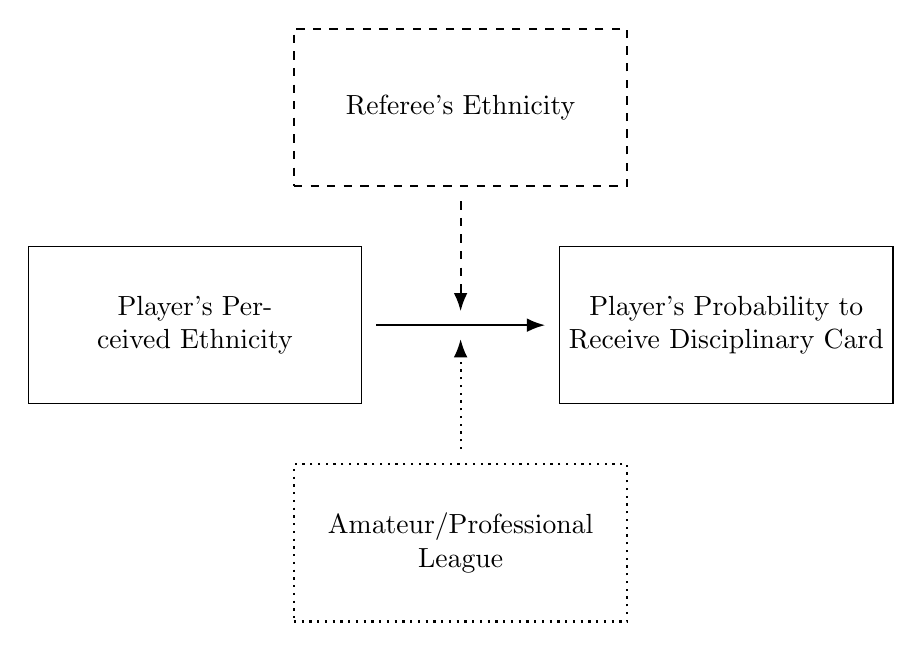
\begin{tikzpicture}[
		node distance = 2.5cm and 2.5cm,
		every node/.style={
			draw,
			rectangle,
			minimum width = 4cm,
			minimum height = 2cm,
			text width = 4cm,
			align=center
		},
		every path/.style={
			draw,	
			-{Latex},
			shorten >=5pt,
			shorten <=5pt}
		]
		
		\node[solid] (A) {Player's Perceived Ethnicity};
		\node[right = of A, solid] (B) {Player's Probability to Receive Disciplinary Card};
		\node[above = 1.75cm of $(A)!0.5!(B)$, dashed, thick] (C)  {Referee's Ethnicity};
		\node[below = 1.75cm of $(A)!0.5!(B)$, dotted, thick] (D) {Amateur/\vspace{0pt}Professional League};
		
		\draw[solid, thick] (A) -- (B);
		\draw[dashed, thick] (C) -- ($(A)!0.5!(B)$);
		\draw[dotted, thick] (D) -- ($(A)!0.5!(B)$);
	\end{tikzpicture}
\end{document}
